\documentclass[11pt]{article}
\usepackage[margin=1.15in]{geometry}
\usepackage{amsmath,amssymb,amsthm}
\usepackage{enumitem}
\usepackage{graphicx}
\usepackage{tikz}
\usetikzlibrary{positioning,fit,arrows}
\usepackage[hidelinks]{hyperref}
\setlength{\parindent}{1.5em}
\setlength{\parskip}{0.3em}
\linespread{1.08}

\newtheorem{proposition}{Proposition}
\theoremstyle{definition}
\newtheorem{definition}{Definition}

\title{Bounded Exposure and the Carrying of Open Claims:\\Trust, Suspicion, and the Allocation of Attention Under Uncertainty}
\author{Flyxion\\\small Independent Researcher}
\date{October 2026}

\begin{document}
\maketitle

\begin{abstract}
\noindent Trust, suspicion, and a large part of ordinary mental life share a structure: an agent with finite attention must carry many claims whose truth or outcome is not yet settled, and must decide how much weight to place on each. This essay develops a stylized model of that structure. Trust is formalized as a policy of acting on unverified claims within a bound on exposure. Under that policy, independence among claims yields a concentration guarantee on total loss, while correlation among claims caps the benefit of diversification at the reciprocal of the correlation. Suspicion is rational when appearances underdetermine causes, and becomes a failure mode in three distinguishable ways: updates scaled to the vividness of evidence instead of its tested reach, an inflated belief in a single shared cause among claims, and the lock-in of attention on one intractable item. A dynamical model of attention share shows a threshold in the amount of concurrent tractable demand below which lock-in is unavoidable and above which it is a recoverable state with a finite basin. Three policies toward others are compared: unconditional trust, as in the Adlerian dialogue literature; bounded exposure; and the strategic cynicism of the Chinese treatise on thick faces and black hearts. A case from a credential market with verification asymmetry illustrates how warrant for claims can be moved from unverifiable lineage to checkable outcomes. The essay then states, as hypotheses with explicit falsifiers, what the model implies for mental health, and sets out what it does not claim. It is a model and not a clinical account, and it offers no guidance for treatment.
\end{abstract}

\section{Introduction}

Three subjects that are usually treated separately turn out to share a mathematical skeleton. The first is trust, which in the organizational and sociological literatures is defined as a willingness to be vulnerable to another party on the basis of expectations about that party's conduct \cite{mayer1995} or as a way of reducing the complexity of a world that cannot be fully verified \cite{luhmann1979}. The second is suspicion, including its pathological forms, which is concerned with the question of when a claim about hidden intent or hidden cause should be believed. The third is the ordinary management of attention across a life containing more unresolved matters than any one mind can hold at once. In each case an agent with limited attention and limited verification capacity must carry claims whose status is open, and the quality of the outcome depends on how weight is distributed among those claims and on how large a loss any single claim is permitted to inflict.

The essay's central proposal is that this distribution of weight can be stated precisely enough to be examined. The proposal is a model, and the model is deliberately stylized. It treats mental health only as an application domain, and the claims it makes about that domain are conditional and carry stated falsifiers. It does not diagnose, it does not recommend treatment, and it takes no position on the causes of any particular condition. Where clinical and psychological literatures are cited, they are cited as sources of empirical regularities with which the model is or is not consistent, and the reader should treat the model as a way of organizing questions and not as an established result.

The argument proceeds in a definite order. Section~\ref{sec:items} defines open items and attention allocation. Section~\ref{sec:trust} formalizes trust as bounded exposure and proves two small results about the benefit of diversifying exposure and the limit that correlation imposes. Section~\ref{sec:policies} compares three policies toward others, drawing on an Adlerian popular literature, on a classical Chinese treatise of strategic cynicism, on popular writing about nonchalance, and on the bounded policy. Section~\ref{sec:credential} applies the framework to a credential market in which the quality of a provider cannot be observed directly. Section~\ref{sec:paranoia} treats suspicion and its failure modes. Section~\ref{sec:lockin} gives a dynamical model of attention lock-in. Section~\ref{sec:multiplexing} separates structured multiplexing from fragmentation and relates the model to existing findings. Sections~\ref{sec:application} and~\ref{sec:limits} state the hypotheses the model implies for mental health, the observations that would count against it, and the limits of the whole enterprise.

\section{Open Items and the Allocation of Attention}
\label{sec:items}

An \emph{open item} is a claim or task whose resolution is pending and whose resolution matters to the agent. The matter may be a prediction about another person's conduct, a worry about a possible event, a project with unfinished stages, or an obligation awaiting action. Each open item $i$ has a stake $\ell_i\ge 0$, the loss the agent would bear if the item resolved adversely, and a degree of tractability, by which is meant the extent to which further attention to the item advances its resolution. A project with identifiable next steps is tractable. A worry about an event that cannot be influenced, or about the private intentions of another party that cannot be verified, is intractable in this sense, since additional attention does not change what will happen or what can be known.

The agent has a finite attention budget, normalized to one, and allocates a share $w_i\ge 0$ to each open item with $\sum_i w_i=1$. The degree to which attention is concentrated is measured by the Herfindahl index
\begin{equation}
H(w)\;=\;\sum_i w_i^{2},
\label{eq:herfindahl}
\end{equation}
which equals $1/n$ when attention is spread equally over $n$ items and equals one when a single item absorbs all attention. Sustained values of $H$ near one will be called \emph{lock-in}. Lock-in on a tractable item is unremarkable and is often what focused work looks like. Lock-in on an intractable item is the case of interest, since attention is then consumed without advancing resolution.

Two features of this setup deserve comment. The first is that the allocation of attention is not wholly under voluntary control, and the model accordingly allows the share an item receives to depend on a demand, or salience, that the item exerts, and which may itself depend on how much attention it has received. The second is that the model makes no assumption about the content of the items. A claim about a neighbour, a task in a workshop, and a fear about the future are all open items, and the model distinguishes them only by stake and tractability. This neutrality is a modelling choice and is not a claim that the items are psychologically equivalent.

\section{Trust as Bounded Exposure}
\label{sec:trust}

The organizational definition of trust as a willingness to be vulnerable \cite{mayer1995} suggests a quantity that can be bounded. Let an agent act on claim $i$ without verifying it, and let $a_i\in[0,1]$ be the fraction of the agent's action that depends on that claim. The \emph{exposure} to claim $i$ is
\begin{equation}
e_i\;=\;\ell_i\,a_i,
\label{eq:exposure}
\end{equation}
the loss the agent would bear if the claim were false, weighted by the degree of reliance. A policy of \emph{bounded exposure} acts on an unverified claim only when $e_i\le\bar e$ for a bound $\bar e$ chosen by the agent, and otherwise either verifies the claim at cost $c_i$ or declines to rely on it. When the claim has credence $p_i$ and verification would remove the loss, verification is worthwhile when $c_i<(1-p_i)\,\ell_i$, and the bound $\bar e$ is the point beyond which the agent will not rely on an unverified claim even when verification is expensive.

The practical value of the bound is that it permits an agent to rely on many unverified claims at once while controlling the total loss. This can be stated as a concentration result.

\begin{proposition}[Diversified exposure]
Let $X_1,\dots,X_n$ be independent random losses with $0\le X_i\le b_i$, let $S=\sum_i X_i$, and let $t>0$. Then
\begin{equation}
\Pr\bigl(S-\mathbb E[S]\ge t\bigr)\;\le\;\exp\!\left(-\frac{2t^{2}}{\sum_i b_i^{2}}\right).
\label{eq:hoeffding}
\end{equation}
In particular, if total exposure $B=\sum_i b_i$ is fixed, the bound is strongest when exposure is spread equally, $b_i=B/n$, where $\sum_i b_i^2=B^2/n$, and is weakest when it is concentrated in one claim, where $\sum_i b_i^2=B^2$. Spreading therefore improves the exponent by a factor of $n$.
\end{proposition}

\begin{proof}
Inequality~\eqref{eq:hoeffding} is Hoeffding's inequality for sums of independent bounded random variables \cite{hoeffding1963}. For fixed $B$ and $\sum_i b_i=B$, the quantity $\sum_i b_i^2$ is minimized at equal $b_i$ by the Cauchy--Schwarz inequality and maximized when a single $b_i$ equals $B$.
\end{proof}

The proposition says that bounding the exposure to each claim is what makes it safe to rely on many of them, and that trust extended to a large number of independent parties is less risky in the aggregate than trust concentrated on one. The qualification is independence, and independence is exactly what suspicion tends to deny. Suppose the losses share a common cause, so that the claims are exchangeable with pairwise correlation $\rho$ and common variance $\sigma^2$. Then
\begin{equation}
\operatorname{Var}(S)\;=\;n\sigma^{2}\bigl(1+(n-1)\rho\bigr)\;=\;\frac{n^{2}\sigma^{2}}{n_{\mathrm{eff}}},\qquad n_{\mathrm{eff}}\;=\;\frac{n}{1+(n-1)\rho}.
\label{eq:neff}
\end{equation}

\begin{proposition}[Correlation caps diversification]
For fixed $\rho>0$ the effective number of independent claims $n_{\mathrm{eff}}$ is increasing in $n$ and satisfies $n_{\mathrm{eff}}\to 1/\rho$ as $n\to\infty$. At $\rho=1$, $n_{\mathrm{eff}}=1$ for every $n$.
\end{proposition}

\begin{proof}
Differentiating $n/(1+(n-1)\rho)$ in $n$ gives $(1-\rho)/(1+(n-1)\rho)^2\ge 0$. The limit follows by dividing numerator and denominator by $n$. At $\rho=1$ the denominator equals $n$.
\end{proof}

Correlation therefore imposes a ceiling on what diversification can achieve: with a pairwise correlation of one tenth, no number of claims behaves like more than ten independent ones, and with a correlation of one, any number of claims behaves like a single claim. The correlation $\rho$ is partly a fact about the world and partly a belief of the agent about the world, and a belief that unrelated events share a single hidden cause sets $\rho$ near one in the agent's own model whatever the true dependence may be.

\section{Three Policies Toward Others}
\label{sec:policies}

The bounded policy is one point in a family. At one end is unconditional trust, which in the model corresponds to $\bar e=\infty$: the agent acts on claims without regard to the loss a false claim would inflict. At the other is the cynical policy, which corresponds to $\bar e=0$ together with a belief that $\rho$ is near one: the agent relies on no unverified claim and interprets claims as instances of a single underlying strategic motive. Figure~\ref{fig:policies} places the three along the exposure axis.

\begin{figure}[htbp]
\centering
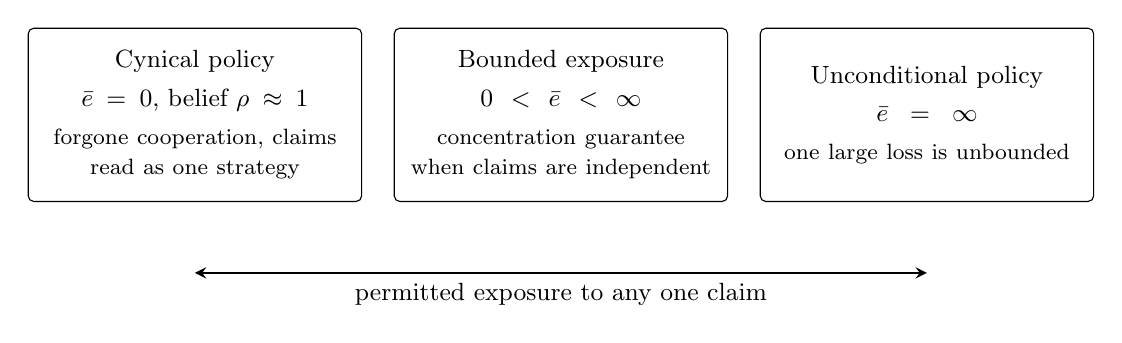
\begin{tikzpicture}[
    node distance=4mm,
    box/.style={draw, rounded corners=2pt, align=center, minimum height=22mm, text width=40mm, font=\small},
    arr/.style={stealth-stealth, thick}
]
\node[box] (cyn) {Cynical policy\\[1mm]$\bar e=0$, belief $\rho\approx 1$\\[1mm]\footnotesize forgone cooperation, claims read as one strategy};
\node[box, right=of cyn] (bnd) {Bounded exposure\\[1mm]$0<\bar e<\infty$\\[1mm]\footnotesize concentration guarantee when claims are independent};
\node[box, right=of bnd] (unc) {Unconditional policy\\[1mm]$\bar e=\infty$\\[1mm]\footnotesize one large loss is unbounded};
\draw[arr] ([yshift=-9mm]cyn.south) -- ([yshift=-9mm]unc.south) node[midway, below, font=\small] {permitted exposure to any one claim};
\end{tikzpicture}
\caption{Three policies toward unverified claims, arranged by the bound on exposure to any single claim. Only the middle policy has both a loss guarantee and the benefits of cooperation.}
\label{fig:policies}
\end{figure}

The unconditional pole is represented in a widely read popular literature on Adlerian psychology, in the dialogues of Kishimi and Koga \cite{kishimi2013, kishimi2016}, which present themes from Alfred Adler's individual psychology \cite{ansbacher1956} in a Japanese philosophical-dialogue form. Two themes bear on the present model. The first is the separation of tasks, which holds that each person's responsibilities are identified by asking who bears the consequences of a choice, so that other people's reactions to one's choices are their own task and not one's own. In the vocabulary of open items this is a rule of admission: it removes from the agent's list the items whose resolution depends wholly on another party, and in particular the approval and disapproval of others. The second is the regard for others as a stance of belief in persons instead of a conditional calculation about them. These presentations are works of popular philosophy and not clinical research, and their teleological claim that present feelings serve present purposes more than they reflect past causes is contested. For the present purpose only a narrower point is needed. An unconditional regard for persons is compatible with a bounded policy of action on their claims, because regard is a stance toward a person while exposure is a property of reliance on a particular claim. Extending good faith to someone does not require resting a large share of one's welfare on an assertion that one cannot check.

The cynical pole is represented by the early twentieth-century Chinese treatise of Li Zongwu on the thick face and the black heart \cite{li1911, chu1992}. Li treats political life as a contest of concealment and ruthlessness, defining the thick quality as the concealment of one's own will and the black quality as the imposition of one's will on others, and arguing that those who succeed in history are those who practise them most completely. As a text it is polemical and has been read both as satire and as a manual, and it is cited here only as a clear statement of the policy in which every claim is assumed to serve a concealed advantage. In the model that policy has two components. It sets exposure to zero, which forgoes whatever is gained by cooperation. And it sets the believed correlation among claims near one, since all claims are read as expressions of one motive, so that by Proposition~2 the agent's effective number of independent claims is close to one and the information in any additional claim is discounted accordingly. The policy is therefore costly even when it is correct about a particular counterpart, because it forecloses the diversified exposure that Proposition~1 shows to be safe.

The three policies differ in what they require the agent to know. Unconditional trust requires nothing about the counterpart and bears an unbounded risk. Cynicism requires an assumption about every counterpart and bears the costs of isolation. Bounded exposure requires an estimate of the loss that a false claim would inflict and a choice of how much of that loss to accept, which is a smaller informational demand than either alternative and is the one that can be meaningfully revised as evidence arrives.

Popular writing on nonchalance shows a fourth position that the model separates into two quite different things. One strand describes an interpersonal posture of performed indifference, in which delayed replies, sarcasm, and feigned boredom conceal that the agent cares \cite{baltimore2025, providence2025}. In the model this is not a low stake. The agent's true stake $\ell_i$ is unchanged and only the displayed stake is set near zero, so the counterpart cannot read the signal and both sides may withhold, which is a coordination failure in the exposure each is willing to show. Those sources attribute the pattern to the permanence and audience of online disclosure and to an intolerance of earnestness, and they assert mental-health costs without citing studies; they are used here only as a description of the phenomenon, and the causal and clinical claims are not adopted. The other strand defends nonchalance as a genuine detachment from outcomes that reduces stress \cite{alwani}. In the model that corresponds to actually lowering the stake or the attention weight on an item, and it is the intended effect of the Adlerian separation of tasks, in which an outcome that lies in another person's hands is not carried as one's own open claim. The two differ in what they do to $\ell_i$. Performed indifference leaves it high and hides it; genuine detachment lowers it. The model therefore predicts that only the second reduces the load of open items, and that the first adds the cost of maintaining a display on top of an unchanged load.

\section{A Credential Market with Verification Asymmetry}
\label{sec:credential}

A concrete case clarifies how the framework applies when the quality of a provider cannot be observed directly. Public warning pages of a certain genre circulate in craft and martial traditions, written by senior practitioners and addressed to prospective students. One such page, written by a senior student of a Chinese martial art, asserts that few people in the world know the art in full, that many who teach it have trained only briefly, that a particular curriculum should be completed within a stated period, that certain additions to the art such as extreme flexibility work are not part of it, and that instruction by an unqualified teacher can cause permanent injury to the knees, back, and neck. It lists signs by which a prospective student can judge a teacher, including how long the teacher has trained, whether the teacher knows more than one form, whether movements show real power, and whether the teacher screams throughout a form. It also notes that the author's own instructional materials are what would supply the missing forms.

The page is useful as evidence about the structure of the market without being treated as a verdict on any individual, and the claims it makes about particular persons are not assessed here. The structure has several features. The decisive facts, such as who trained for how long and who learned what, are held privately by a small group, and the page appeals to that private knowledge, saying in effect that the lineage holder knows exactly how long each person studied. A prospective student cannot verify those facts and so is asked to trust the author's account of who is trustworthy. The author has an interest in the outcome, since the competing teachers are also competitors for students and for the sale of materials, and the page says so in passing. The warning signs offered are proxies, of the sort that are easy to state and imperfectly correlated with quality, and screams throughout a form or the inclusion of flexibility work might coincide with poor instruction, with a legitimate variant of the art, or with neither.

In the vocabulary of exposure the case is instructive. The losses are real and are of two kinds, money and bodily injury, and the second is large and sometimes irreversible, so that $\ell_i$ is high. The first response suggested by the model is to bound exposure at entry: begin with short, low-cost, reversible commitments before relying on a provider for extended or physically demanding instruction. The second is to move the warrant for the claim from a source that cannot be checked to one that can. The question of the teacher's lineage is a claim about a private record. The question of whether instruction is safe is largely observable by the student and by third parties: whether joint loading is progressive, whether drills are explained, whether pain in the knees or back is treated as a signal to stop, and whether other students are injured. Safety practices are checkable in a way that lineage is not. This is the same move that the money essay of this series makes when it replaces a valuation that cannot be verified with the attestation of a transformation that can, and it is an instance of a general principle: where the decisive fact is private, trust should be anchored to claims whose warrant is public, and where warrant must come from an interested party, exposure should be bounded until independent evidence accumulates.

Two further literatures bear on the question of whose claims are admitted to the list of things believed. The concept of epistemic trust, proposed in the psychotherapy literature, concerns the willingness to treat information from another as reliable and personally relevant, and has been proposed as a mechanism by which therapeutic relationships work \cite{fonagy2014}. The concept of testimonial injustice, from social epistemology, concerns the systematic discounting of some speakers' credibility for reasons unrelated to the quality of what they say \cite{fricker2007}. Both identify admission policy as the point of leverage: not merely how much weight a claim receives once admitted, but which claims are admitted at all, and for whom.

\section{Suspicion and Its Failure Modes}
\label{sec:paranoia}

Suspicion begins as a rational response to a fact about the world: appearances underdetermine causes. A given observation is compatible with a very large number of causal histories, and no agent can evaluate them all. Withholding full trust from claims that cannot be checked is not a defect. What distinguishes a functioning suspicion from a destructive one is not whether it is present but how it behaves, and three failure modes can be separated, each corresponding to one component of the model.

The first is an error in the update rule. Let an agent's log-odds on a hypothesis change by $\Delta$ on receiving new evidence. A disciplined rule bounds the change by the tested evidentiary reach $R$ of the evidence, that is, by the extent to which the evidence has survived independent corroboration, cross-examination, and consideration of alternatives:
\begin{equation}
|\Delta|\;\le\;\lambda\,R .
\label{eq:update}
\end{equation}
The failure is an update that scales instead with the vividness of the evidence, the extent to which it is salient, emotionally charged, or narratively coherent, regardless of how much of it has been tested. This is the principle that legal procedure embodies when it requires disclosure, cross-examination, burdens of proof, and review: it constrains the update rule, so that new evidence can revise judgment without being permitted to rewrite the entire interpretive structure at once.

The second failure is an inflated belief in a shared cause. If an agent comes to believe that many separate observations are expressions of a single hidden agency, then by Proposition~2 the agent's effective number of independent claims falls toward one, and each new observation is treated as confirming the same hypothesis instead of as an independent test of it. In such a state evidence that would ordinarily disperse the weight of belief across alternatives instead concentrates it. The third failure is lock-in in the sense of Section~\ref{sec:items}: attention concentrates on the suspected threat to the exclusion of other items, and because the threat is intractable, more attention does not resolve it.

These three failures are conceptually separable and can occur singly. A person with an accurate update rule may still allocate too much attention to a real but unresolvable threat, and a person with a distributed allocation may still hold a mistaken belief about the dependence among events. Their joint presence is what makes the condition self-sustaining, and the cognitive literature on persecutory ideas has described processes of this general kind, including worry, biases in how much evidence is gathered before a conclusion is drawn, and behaviours that protect against the feared outcome while preventing its disconfirmation \cite{freeman2007}. The model does not diagnose any person or condition and should not be used to do so. Its purpose is to state the differences among the failures precisely, so that questions about which is operating in a given case can be asked at all.

\section{A Model of Attention Lock-In}
\label{sec:lockin}

The relation between attention share and salience can be given a minimal dynamical form. Let one intractable item have demand $d\ge 0$, and let the remaining items be tractable, with total demand $M>0$ that is held constant over the period of interest. Attention is allocated in proportion to demand, so that the intractable item receives the share
\begin{equation}
w\;=\;\frac{d}{d+M}.
\label{eq:share}
\end{equation}
The demand of the intractable item evolves according to
\begin{equation}
\dot d\;=\;-\gamma\,d\;+\;s\;+\;\eta\,d\,w,
\label{eq:dynamics}
\end{equation}
where $\gamma>0$ is a rate of decay or resolution, $s>0$ a constant inflow of salience, and $\eta>0$ a feedback gain by which attention paid to the item increases its salience. The feedback term represents the observation, common in the literature on repetitive negative thought, that attending to a worry in an abstract and evaluative mode tends to prolong it \cite{nolen1991, watkins2008}. The decay term represents closure, including the effect of having a plan, which has been reported to reduce the intrusion of unfinished goals without requiring their completion \cite{masicampo2011}. The tractable items appear only through $M$, since they draw attention but do not feed back into the demand of the intractable item.

Multiplying~\eqref{eq:dynamics} by $d+M$ shows that $\dot d=N(d)/(d+M)$ with
\begin{equation}
N(d)\;=\;(\eta-\gamma)\,d^{2}+(s-\gamma M)\,d+sM,
\label{eq:numerator}
\end{equation}
so the equilibria are the nonnegative roots of $N$ and their stability is read from the sign of $N$ on either side.

\begin{proposition}[Thresholds in concurrent tractable demand]
\emph{(a)} If $\eta<\gamma$, there is exactly one positive equilibrium $d^{*}$, it is stable, and for large $M$ its attention share satisfies $w^{*}\approx s/(\gamma M)$, which tends to zero as $M\to\infty$.

\emph{(b)} If $\eta>\gamma$, define
\begin{equation}
M_{\mathrm{crit}}\;=\;\frac{s\,\bigl(\sqrt{\eta}+\sqrt{\eta-\gamma}\bigr)^{2}}{\gamma^{2}}.
\label{eq:mcrit}
\end{equation}
If $M<M_{\mathrm{crit}}$ then $N(d)>0$ for all $d\ge 0$ and demand grows without bound, so that $w\to 1$. If $M>M_{\mathrm{crit}}$ there are two positive equilibria $d_{-}<d_{+}$, where $d_{-}$ is stable and $d_{+}$ is unstable. Initial demand below $d_{+}$ converges to $d_{-}$, and initial demand above $d_{+}$ grows without bound.
\end{proposition}

\begin{proof}
For (a), the leading coefficient of $N$ is negative and $N(0)=sM>0$, so $N$ has exactly one positive root and changes sign there from positive to negative, which is stability. For large $M$ the dominant balance in $N(d)=0$ is $-\gamma M d+sM\approx 0$, giving $d^{*}\approx s/\gamma$ and hence $w^{*}=d^{*}/(d^{*}+M)\approx s/(\gamma M)$. For (b), the leading coefficient is positive and $N(0)=sM>0$. The discriminant of $N$ is $D(M)=\gamma^{2}M^{2}-2s(2\eta-\gamma)M+s^{2}$, with roots $M_{\pm}=s\bigl[(2\eta-\gamma)\pm 2\sqrt{\eta(\eta-\gamma)}\bigr]/\gamma^{2}$, and $(2\eta-\gamma)+2\sqrt{\eta(\eta-\gamma)}=(\sqrt{\eta}+\sqrt{\eta-\gamma})^{2}$, so $M_{+}=M_{\mathrm{crit}}$. For $M<M_{+}$ with $M>M_{-}$ the discriminant is negative and $N>0$. For $M\le M_{-}$ the discriminant is nonnegative but $s-\gamma M>0$, so both roots are negative and again $N>0$ for $d\ge 0$. For $M>M_{+}$ the discriminant is positive and $s-\gamma M<0$, so both roots are positive. Since $N$ is positive at zero and between the roots it is negative, the smaller root is stable and the larger is unstable.
\end{proof}

Proposition~3 states the structure that the earlier sections left informal. When feedback is weaker than decay, additional concurrent tractable demand reduces the attention share of the intractable item smoothly. When feedback exceeds decay, concurrent demand matters in a sharper way: below a critical amount lock-in is unavoidable, and above it the agent has a stable low-share state with a finite basin of attraction, so that a sufficiently large salience shock can still push the system across the unstable equilibrium into runaway. The size of the basin grows with $M$. Figure~\ref{fig:lockin} illustrates the three cases with parameters chosen to display the structure and not estimated from any data.

\begin{figure}[htbp]
\centering
\includegraphics[width=0.88\linewidth]{figures/fig_lockin.png}
\caption{Dimensionless illustrative simulation of attention lock-in with $s=0.10$, $\gamma=0.50$, $\eta=0.80$, for which $M_{\mathrm{crit}}\approx 0.83$. Below the threshold the share runs away without any shock. Above it the system holds a low-share state, and a fixed shock of the same size pushes the case with the smaller basin into lock-in while the case with the larger basin recovers. Curves end where demand has diverged. The simulation shows the structure of the model and does not estimate the size of any effect in any person.}
\label{fig:lockin}
\end{figure}

The model identifies four levers, and they correspond to different families of intervention in the sense that they change different terms. The feedback gain $\eta$ can be lowered by changing the mode in which an item is attended to, and the repetitive-thought literature distinguishes abstract and evaluative processing from concrete and problem-focused processing along roughly these lines \cite{watkins2008}. The decay rate $\gamma$ can be raised by closure, including by plans that do not complete the task but specify when and how it will be addressed \cite{masicampo2011}. The concurrent tractable demand $M$ can be raised by taking on tractable work, which is the structure that behavioural activation approaches to low mood employ, in which the scheduling of engaging activities is a primary component \cite{jacobson1996, dimidjian2006}. The admission of items to the list can be controlled, and the Adlerian separation of tasks is a rule of this fourth kind. The model does not claim that any of these works for any person. It claims that, if the dynamics are even approximately right, they are four distinct ways to move the system, and that they should be distinguishable in evidence.

\section{Structured Multiplexing and Fragmentation}
\label{sec:multiplexing}

The role of $M$ raises the obvious objection that the model seems to recommend more concurrent demand, while a substantial literature associates heavy media multitasking with poorer performance on tasks of cognitive control \cite{ophir2009}. The objection is serious, and the model's reply depends on distinguishing two things that are both called multitasking. The literature on media multitasking measures the habitual consumption of several media streams at once and typically finds correlational associations with attention and memory outcomes, although later reviews describe the evidence as mixed and note that the direction of causation is not established \cite{uncapher2018}. The quantity $M$ in the model is something different. It is the demand of concurrent items that are \emph{tractable}, in the sense that each has its own persistent state and its own next steps, and that the agent has chosen. The distinction is between structured multiplexing, in which several threads of work advance in turn with their state preserved, and fragmentation, in which interruptions generated elsewhere break attention without any corresponding progress on anything.

Fragmentation of this kind adds demand without adding closure, and nothing in the model suggests it should help. Capacity limits also matter. Working memory holds only a small number of items at once \cite{cowan2001}, and the model's treatment of $M$ as a fixed aggregate ignores the costs of switching among threads. The model should therefore be read as applying within the range in which the tractable threads can actually be kept in good order, and as silent about the regime beyond it. This is a real limit and is stated again in Section~\ref{sec:limits}. A companion essay on boredom and constraint develops a related structural account, in which attention is stabilized by narrowing option spaces and by treating situations as problems with structure, and the present model is consistent with that account in treating engagement with tractable structure as a stabilizing term. It is also consistent with the long-standing description of absorption in tasks of matched difficulty as a high-quality form of experience \cite{csikszentmihalyi1990}.

\section{What the Model Implies for Mental Health}
\label{sec:application}

The model supports a modest set of conditional claims, which can be stated as hypotheses together with the observations that would count against each. They are stated at the level of the model's structure and should be understood as research questions.

\begin{enumerate}[leftmargin=2em,itemsep=0.3em]
\item \emph{Attention share and rumination.} Within a person over time, the share of attention on a single intractable item should predict the intensity of repetitive negative thought beyond what overall engagement predicts. The hypothesis fails if overall activity level, with no relation to the concentration of attention, accounts for the association.
\item \emph{Structure versus interruption.} Voluntary, state-preserving multiplexing and externally generated interruption should dissociate in their relation to rumination, with the first associated with lower share on intractable items and the second not. The hypothesis fails if the two behave alike.
\item \emph{Closure without completion.} Specifying a plan for an unfinished goal should reduce its intrusion without requiring the goal to be completed. This regularity has been reported \cite{masicampo2011} and, like most findings from a single research program, deserves independent replication before it is relied on. The hypothesis fails if replication does not support it.
\item \emph{Inflated dependence among claims.} Beliefs that persecute should be associated with an elevated judged dependence among events that are independent in fact. The hypothesis fails if judged dependence does not differ between people holding such beliefs and others.
\item \emph{Lever dissociation.} Interventions that raise $M$ without changing $\eta$ or $\gamma$ should reduce lock-in only to the extent that they move the system above the critical amount in Proposition~3. The hypothesis fails if increases in concurrent tractable demand reduce rumination in the regime where feedback is already strong enough that a modest $M$ cannot help, or fail to reduce it in the regime where the model says they should.
\end{enumerate}

No quantitative prediction is offered, because the model has no estimated parameters and an estimate would require data on individuals that this essay does not use. The hypotheses concern directions and dissociations and not magnitudes.

\section{Limits and Scope}
\label{sec:limits}

Several limits bear on how the essay should be read. The model is stylized. Attention is treated as divisible and allocated in proportion to demand, the demand of the tractable items is held constant, and the switching costs and capacity limits that matter in practice are omitted. The simulation in Figure~\ref{fig:lockin} is a dimensionless illustration and not an empirical fit. Mental health is not reduced here to attention allocation. Many conditions have biological, social, and developmental determinants that the model does not represent, and the essay makes no claim that task load, or the structure of attention, is the cause or the remedy of any of them. It is not a basis for self-treatment, and it does not substitute for clinical care. The sources drawn from the Adlerian popular literature are works of philosophy presented as dialogue and not research reports, and their central teleological claims are contested, while the Chinese treatise is a historical and polemical text whose value here is as a clear statement of a policy and not as evidence about human nature. The case of the credential market is a single illustration drawn from a document written by an interested party, and its claims about particular persons are unverified and have not been assessed. The psychological findings cited, including those on rumination, plan-making, behavioural activation, and media multitasking, vary in strength and in replication status, and are cited as sources of regularities that the model should be compared with, not as established support.

\section{Conclusion}

Trust, suspicion, and the ordinary carrying of unresolved matters can be described as problems of one kind: how an agent with limited attention and limited verification should distribute weight and exposure across claims it cannot settle. Bounded exposure is a policy that makes it safe to rely on many unverified claims at once, provided they are not tied together by a common cause, and the same policy marks the difference between a stance of good faith toward persons and a policy of resting large losses on particular unverified assertions. Suspicion becomes a failure mode in three separable ways, in the scaling of updates, in the belief that events share one cause, and in the concentration of attention on an intractable item, and the dynamics of the last show a threshold in concurrent tractable demand that is sharp when feedback is strong. The framework is useful principally because it makes distinctions that can be tested: between regard for persons and reliance on their claims, between structured multiplexing and fragmentation, and between interventions that move different terms of the same dynamics. It makes no claim about any person's condition and offers no treatment. What it offers is a way of asking, for a given case, which of the weights is out of proportion and why.

\begin{thebibliography}{99}
\bibitem{ansbacher1956} H.~L. Ansbacher and R.~R. Ansbacher (eds.), \emph{The Individual Psychology of Alfred Adler}, Basic Books, 1956.
\bibitem{chu1992} C.-N. Chu, \emph{Thick Face, Black Heart}, Warner Books, 1992.
\bibitem{baltimore2025} Baltimore Therapy Group, ``Understanding the Nonchalance Epidemic,'' therapy blog post, 27 October 2025.
\bibitem{providence2025} Providence Therapy Group, ``Breaking the Nonchalance Trend,'' therapy blog post.
\bibitem{alwani} R.~Alwani, ``The Essential Art of Nonchalance,'' \emph{Medium}, personal essay.
\bibitem{cowan2001} N.~Cowan, ``The Magical Number 4 in Short-Term Memory: A Reconsideration of Mental Storage Capacity,'' \emph{Behavioral and Brain Sciences} 24(1), 2001.
\bibitem{csikszentmihalyi1990} M.~Csikszentmihalyi, \emph{Flow: The Psychology of Optimal Experience}, Harper \& Row, 1990.
\bibitem{dimidjian2006} S.~Dimidjian et al., ``Randomized Trial of Behavioral Activation, Cognitive Therapy, and Antidepressant Medication in the Acute Treatment of Adults With Major Depression,'' \emph{Journal of Consulting and Clinical Psychology} 74(4), 2006.
\bibitem{fonagy2014} P.~Fonagy and E.~Allison, ``The Role of Mentalizing and Epistemic Trust in the Therapeutic Relationship,'' \emph{Psychotherapy} 51(3), 2014.
\bibitem{freeman2007} D.~Freeman, ``Suspicious Minds: The Psychology of Persecutory Delusions,'' \emph{Clinical Psychology Review} 27(4), 2007.
\bibitem{fricker2007} M.~Fricker, \emph{Epistemic Injustice: Power and the Ethics of Knowing}, Oxford University Press, 2007.
\bibitem{hoeffding1963} W.~Hoeffding, ``Probability Inequalities for Sums of Bounded Random Variables,'' \emph{Journal of the American Statistical Association} 58(301), 1963.
\bibitem{jacobson1996} N.~S. Jacobson et al., ``A Component Analysis of Cognitive-Behavioral Treatment for Depression,'' \emph{Journal of Consulting and Clinical Psychology} 64(2), 1996.
\bibitem{kishimi2013} I.~Kishimi and F.~Koga, \emph{The Courage to Be Disliked}, Japanese edition 2013, English translation 2018.
\bibitem{kishimi2016} I.~Kishimi and F.~Koga, \emph{The Courage to Be Happy}, Japanese edition 2016, English translation 2019.
\bibitem{li1911} Z.~Li, \emph{Hou hei xue} (the study of the thick face and the black heart), early twentieth century (commonly dated 1911).
\bibitem{luhmann1979} N.~Luhmann, \emph{Trust and Power}, Wiley, 1979.
\bibitem{masicampo2011} E.~J. Masicampo and R.~F. Baumeister, ``Consider It Done! Plan Making Can Eliminate the Cognitive Effects of Unfulfilled Goals,'' \emph{Journal of Personality and Social Psychology} 101(4), 2011.
\bibitem{mayer1995} R.~C. Mayer, J.~H. Davis, and F.~D. Schoorman, ``An Integrative Model of Organizational Trust,'' \emph{Academy of Management Review} 20(3), 1995.
\bibitem{nolen1991} S.~Nolen-Hoeksema, ``Responses to Depression and Their Effects on the Duration of Depressive Episodes,'' \emph{Journal of Abnormal Psychology} 100(4), 1991.
\bibitem{ophir2009} E.~Ophir, C.~Nass, and A.~D. Wagner, ``Cognitive Control in Media Multitaskers,'' \emph{Proceedings of the National Academy of Sciences} 106(37), 2009.
\bibitem{uncapher2018} M.~R. Uncapher and A.~D. Wagner, ``Minds and Brains of Media Multitaskers: Current Findings and Future Directions,'' \emph{Proceedings of the National Academy of Sciences} 115(40), 2018.
\bibitem{watkins2008} E.~R. Watkins, ``Constructive and Unconstructive Repetitive Thought,'' \emph{Psychological Bulletin} 134(2), 2008.
\end{thebibliography}

\end{document}
